\documentclass{standalone}
\usepackage{tikz}
\usepackage{ctex,siunitx}
\usepackage{tkz-euclide}
\usepackage{amsmath}
\usetikzlibrary{patterns, calc}
\usetikzlibrary {decorations.pathmorphing, decorations.pathreplacing, decorations.shapes,decorations.markings,positioning, snakes}

\begin{document}
\small
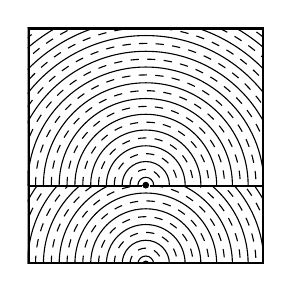
\begin{tikzpicture}[>=stealth]
  \clip (-1.5, 0) rectangle (1.5,3);
  \foreach \x in {.1,.3,...,2}
  {
      \draw (-\x,0) arc (180:0:\x);
  }
  \foreach \x in {.2,.4,...,2}
  {
  	\draw [dashed]  (-\x,0) arc (180:0:\x);
  }
  \draw[ultra thick] (-1.5,1)--(-.05,1);
  \draw[ultra thick] (1.5,1)--(.05,1);
  \fill [white](-1.5,1) rectangle (1.5, 2.2);
  \foreach \x in {.1,.3,...,3}
  {
      \draw (-\x,1) arc (180:0:\x);
  }
 \foreach \x in {.2,.4,...,3}
 {
 	\draw [dashed]  (-\x,1) arc (180:0:\x);
 }
  \draw  [fill=black] (0,1)  circle (1pt);
  \draw[ultra thick] (-1.5, 0) rectangle (1.5,3);
  \draw  [fill=black] (0,0)  circle (1pt);
\end{tikzpicture}
\end{document}